\section{Search-based methods}

Search-Based Planning Algorithms are straightforward, versatile, and offer valuable theoretical guarantees when connectivity assumptions are met.

These algorithms are well-suited for composite maps, but also to free space representation. 
Considering a cell on the grid, we have a total of eight connectivity: four diagonal and four orthogonal
\begin{figure}[H]
    \centering
    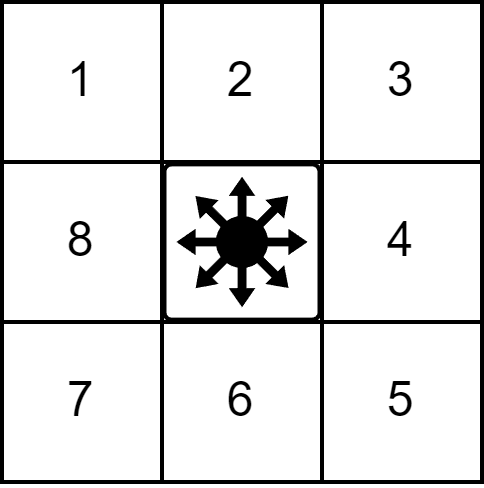
\includegraphics[width=0.25\linewidth]{images/gmc.png}
    \caption{Grid map cells connectivity}
\end{figure}
The general concept involves:
\begin{enumerate}
    \item Creating a discretized representation of the planning problem.
    \item Constructing a graph based on this discretized representation, often using 4 or 8 neighbors connectivity.
    \item Searching the graph to find the optimal solution.
\end{enumerate}
Optionally, integrating the construction of the representation with the search process, only generating what is required at each step.

\paragraph*{Robot shape}
Modeling a real mobile robot as a point isn't practical; instead, its shape is considered, and obstacles are expanded accordingly. 
However, this approach introduces challenges and necessitates a trade-off between memory usage and performance.

\paragraph*{Configuration space}
To achieve precise collision detection, the configuration space is employed, where a configuration of an object is denoted by a point $q=(q_1,q_2,\cdots,q_n)$. 
A point $q$ is considered free if the robot positioned at $q$ doesn't collide. 
\begin{definition}[\textit{C-obstacle}]
    C-obstacle is the union of all points $q$ where the robot collides.
\end{definition}
\begin{definition}[\textit{C-fredd}]
    C-free is the union of all points $q$ where the robot does not collide.
\end{definition}
Hence, we define
\[\text{C-space}=\text{C-free}\cup \text{C-obstacle}\]
Planning tasks can be executed within C-Space. 

A robot is capable of both translation and rotation within the plane. 
To accommodate this movement, obstacles need to be enlarged based on the orientation of the robot.

\paragraph*{Algorithms}
Various algorithms are at disposal:
\begin{itemize}
    \item Some provide the optimal path (e.g., Dijkstra, $\text{A}^\ast$).
    \item Others yield an $\varepsilon$ sub-optimal path (e.g., weighted $\text{A}^\ast$, $\text{ARA}^\ast$, $\text{AD}^\ast$, $\text{R}^\ast$, $\text{D}^\ast$ Lite).
\end{itemize}


\paragraph*{Graph-Based path-finding for minimizing costs}
The objective is to search a graph to find the path that minimizes costs.
\begin{figure}[H]
    \centering
    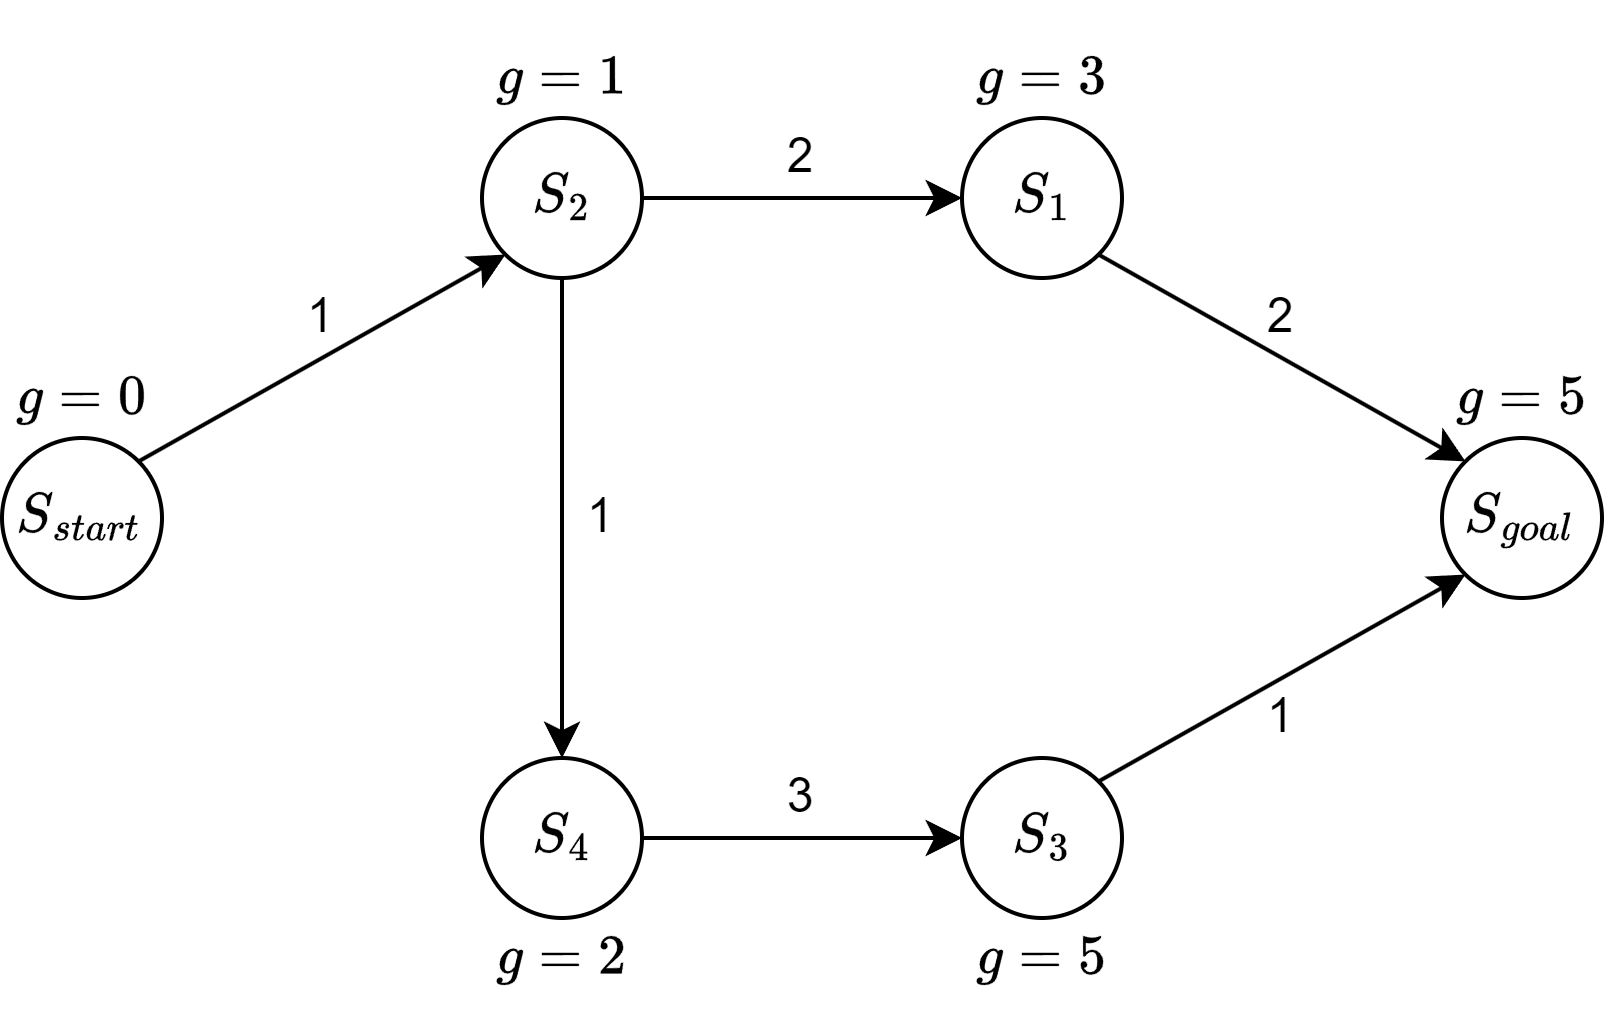
\includegraphics[width=0.5\linewidth]{images/sg.png}
    \caption{Searching graph}
\end{figure}
Numerous search algorithms calculate optimal g-values for pertinent states. 
The function $g(s)$ estimates the cost of the least-cost path from the starting state $s_{\text{start}}$ to $s$. 
The optimal values of this function satisfy:
\[g(s)=\min_{s^{\prime\prime} \text{ in }pred(s)}g(s^{\prime\prime})+c(s^{\prime\prime},s)\]
The least-cost path is determined by backtracking: begin with $s_{\text{goal}}$ and from any state $s$, move to the predecessor state $s^\prime$ such that:
\[s^\prime=\argmin_{s^{\prime\prime} \text{ in }pred(s)}g(s^{\prime\prime})+c(s^{\prime\prime},s)\]

\subsection*{$\text{A}^\ast$ search algorithm}
$\text{A}^\ast$ accelerates the search process by computing $g$-values as follows:
\begin{itemize}
    \item A function $g(s)$ corresponding to the cost of the shortest path found so far from $s_{\text{start}}$ to $s$ found so far.
    \item A function $h(s)$ estimating the cost of the shortest path from $s$ to $s_{\text{goal}}$. 
\end{itemize}
The heuristic function must meet the following criteria:
\begin{itemize}
    \item \textit{Admissible}: for every state $s$ we have that $h(s)\leq c^{\ast}(s,s_{\text{goal}})$. 
    \item \textit{Consistent}: it satisfies the triangle inequality:
        \begin{itemize}
            \item $h(s_{\text{goal}},s_{\text{goal}}) = 0$
            \item For every $s\neq s_{\text{goal}}$, $h(s) \leq c(s,succ(s)) + h(succ(s))$
        \end{itemize}
\end{itemize}
Admissibility follows from consistency, and often vice versa.
\begin{property}
    When the heuristic is both admissible and consistent, $\text{A}^\ast$ becomes optimal.
\end{property}

\begin{algorithm}[H]
    \caption{$\text{A}^\ast$ algorithm}
        \begin{algorithmic}[1]
            \State{$g(s_{\text{start}})=0$}
            \State{All other $g$-values are infinite}
            \State{$\text{OPEN}=\left\{s_{\text{start}}\right\}$}
            \While{$s_{\text{goal}}$ is not expanded}
                \State{Remove $s$ with the smallest $f(s)=g(s)+h(s)$ from OPEN}
                \State{Insert $s$ into CLOSED}
                \For{every successor $s^\prime$ of s such that $s^\prime$ not in CLOSED}
                    \If{$g(s^{\prime}) > g(s) + c(s,s^{\prime})$}
                        \State{$g(s^{\prime}) = g(s) + c(s,s^{\prime})$}
                        \State{insert $s^{\prime}$ into OPEN}
                    \EndIf
                \EndFor 
            \EndWhile
        \end{algorithmic}
\end{algorithm}

\paragraph*{Properties}
$\text{A}^\ast$ ensures:
\begin{itemize}
    \item The return of an optimal solution path.
    \item A minimally required number of state expansions.
\end{itemize}
Regarding state expansion:
\begin{itemize}
    \item Dijkstra's algorithm expands states based on the order of $f=g$ values (approximately).
    \item $\text{A}^\ast$ Search expands states based on the order of $f=g+h$ values.
    \item Weighted $\text{A}^\ast$ expands states according to $f=g+\varepsilon h$ values, where $\varepsilon>1$ introduces a bias towards states closer to the goal.
\end{itemize}
In many domains, Weighted $\text{A}^\ast$ Search has been demonstrated to be significantly faster than $\text{A}^\ast$ by orders of magnitude.

\paragraph*{Variations}
We have several variations, such as: 
\begin{itemize}
    \item AR$\text{A}^\ast$ (Anytime Repairing $\text{A}^\ast$):
        \begin{itemize}
            \item Subsequent queries with decreasing sub-optimality factor $\varepsilon$.
            \item Fast initial (suboptimal) solution.
            \item Refinement over time.
        \end{itemize}
    \item D*/D*-Lite: re-use parts of the previous query and only repair solution locally where changes occurred.
    \item Anytime D* (D* + AR$\text{A}^\ast$): anytime graph-search re-using previous query.
\end{itemize}

\subsection{Summary}
Elements of a Search-based planner:
\begin{itemize}
    \item Graph construction: determines successor states for a given state.
        The graph can be constructed using motion primitives, offering several advantages such as a sparse graph, feasible path generation, and the ability to incorporate various constraints.
        However, a drawback is the potential for incompleteness.
    \item Cost function: associates a cost with each transition in the graph.
    \item Heuristic function: provides estimates of the cost-to-goal.
    \item Graph search algorithm: executes the search process (e.g., A* search).
\end{itemize}
Additionally, the graph can incorporate robot dynamics or kinematics constraints.

\subsection{State-lattice planning}
State-Lattice planning involves motion planning for constrained platforms by conducting a graph search in state-space. 
The process typically includes:
\begin{enumerate}
    \item Discretizing the state-space into a hypergrid (e.g., $x,y,\theta,\kappa$). 
    \item Determining the neighborhood set by connecting each tuple of states with feasible motions.
    \item Defining the cost function or edge weights.
    \item Executing any graph-search algorithm to discover the lowest-cost path.
\end{enumerate}
The benefits of State-Lattice planning include achieving resolution completeness and enabling feasible optimal offline computations owing to its regular structure.
Drawbacks include the curse of dimensionality, where the number of states exponentially increases with the dimensionality of the state-space. 
State-lattice construction necessitates solving nontrivial two-state boundary value problems.
Regular discretization may encounter challenges in narrow passages not aligned with the hypergrid, and discretization can cause discontinuities in state variables not accounted for in the hypergrid, thereby rendering motion plans non-executable.

To address these challenges, minimal neighborhood sets should be designed, avoiding the insertion of edges that can be decomposed with existing controls. 
Decomposition should be close in cost-space.

\paragraph*{Hybrid A*}
Hybrid A* generates motion primitives by sampling the control space, eliminating the need to solve boundary value problems. 
Continuous states resulting from this process are then associated with discrete states in the hypergrid. 
Each grid cell stores a continuous state.
However, there is no longer a guarantee of completeness due to changes in the reachable state space and the pruning of continuous-state branches.